\begin{figure}[htbp]
	\centering
	\begin{tikzpicture}[
			font=\small,
			component/.style={
					draw,
					rounded corners=2pt,
					line width=0.6pt,
					minimum height=2.8cm,
					align=center
				},
			flow/.style={->, line width=0.6pt},
			flowlabel/.style={font=\scriptsize, align=center},
			boundary/.style={densely dashed, line width=1pt, gray}
		]
		\node[component, minimum width=3.2cm] (unity) at (4,0) {Unity};
		\node[component, minimum width=3.6cm] (pipeline) at (10.2,0) {LLM-Pipeline};

		\draw[boundary] (5.95,-2.0) -- (5.95,2.0);

		\node[align=center, label=below:Benutzer*in] (user) at (0,0) {\Huge\faIcon[solid]{user}};
		\coordinate (userPort) at (user.east);

		\draw[flow] (userPort) -- node[above, flowlabel] {Eingabe} (unity.west);
		\draw[flow] ([yshift=0.65cm]unity.east) -- node[pos=0.65, above, flowlabel] {Szenendaten} ([yshift=0.65cm]pipeline.west);
		\draw[flow] ([yshift=-0.65cm]pipeline.west) -- node[pos=0.35, below, flowlabel] {Spezifikation} ([yshift=-0.65cm]unity.east);
	\end{tikzpicture}
	\caption{Systemkontextdiagramm des VSG.}\label{fig:systemkontextdiagramm_vsg_tikz}
\end{figure}
